%----------------------------------------------------------------------------
\chapter{Hallgatói értékelési rendszer}\label{chapter:assessments}
%----------------------------------------------------------------------------

A korábban leírtaknak megfelelően a JPorta tárgyaiban lehetőség van különböző értékeléseket felvenni, majd azokat kurzusokhoz rendelni. Ezeket hozzárendelés után a kurzus oktatói tudják értékelni (\ref{fig:jporta_course_results}. ábra).

Új értékelést csak a tárgy adminisztrátorai tudnak létrehozni és kurzusokhoz rendelni. Az ehhez tartozó felület \aref{fig:jporta_add_result}. ábrán látható. Minden értékeléshez az alábbi tulajdonságok tartoznak:
\begin{itemize}
    \item Név: rövid név, mely azonosítja az értékelést, pl. ZH 1
    \item Típus: előre definiált értékek, melyekhez tartozik egy reguláris kifejezés \cite{RegExp}. Csak olyan értéket vehet fel, ami illeszkedik a hozzá tartozó kifejezésre.
    \item Súly: meghatározza a sorrendet az értékelések megjelenítésénél.
    \item Ki értékelheti: kurzusokhoz, vagy csak a tárgyhoz rendelt oktatók értékelhetik.
    \item Dinamikus-e: az adott értékelés dinamikusan értékelődik-e ki, ld. \aref{section:dynamic-assessments} pontban.
    \item Privát-e: a privát értékeléseket csak az oktatók látják, a hallgatók nem.
    \item Megjegyzés: részletes leírása az értékelésnek, tipikusan dinamikus értékelések esetén hasznos.
    \item Kurzusok: tárgyon belül mely kurzusokhoz akarjuk hozzárendelni az értékelést.
\end{itemize}

\begin{figure}[h]
    \centering
    \resizebox{\textwidth}{!}{
        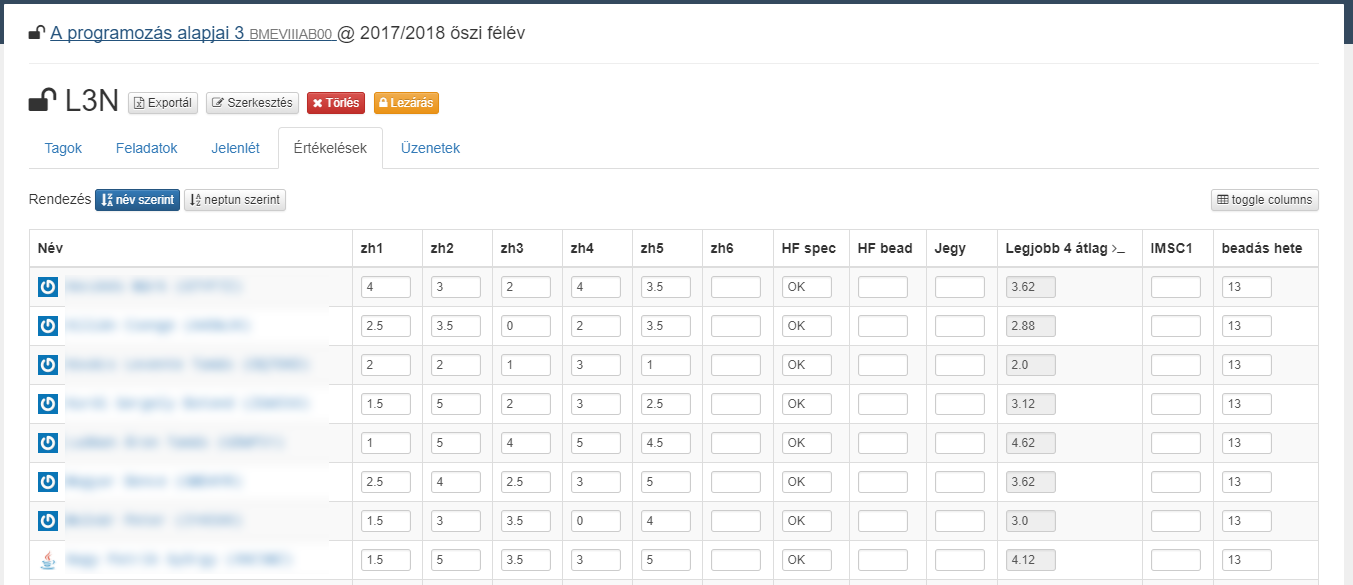
\includegraphics[]{jporta_course_results.png}
    }
    \caption{Hallgatók értékelései}
    \label{fig:jporta_course_results}
\end{figure}

Ezen tulajdonságoknak köszönhetően az értékeléseket egyszerűen és személyreszabhatóan lehet kezelni. Alapvető céljuk a zárthelyi számonkérések eredményének adminisztrálása, de bármikor hozzáadhatunk egyéb mezőket is. Ilyen lehet pl. a hallgató házi feladatának személyes bemutatására kijelölt időpont, vagy éppen a házi feladat dokumentáció státusza.

Az univerzalitás egyedüli határa a megfelelő típus megtalálása az értékeléshez, de ez könnyen bővíthető. Új igény felmerülésekor a portál adminisztrátorai hozzáadhatnak új típust, mely egy tetszés szerinti reguláris kifejezésre illeszkedő tartalmat vár.

\begin{figure}[p]
    \centering
    \resizebox{0.9\textwidth}{!}{
        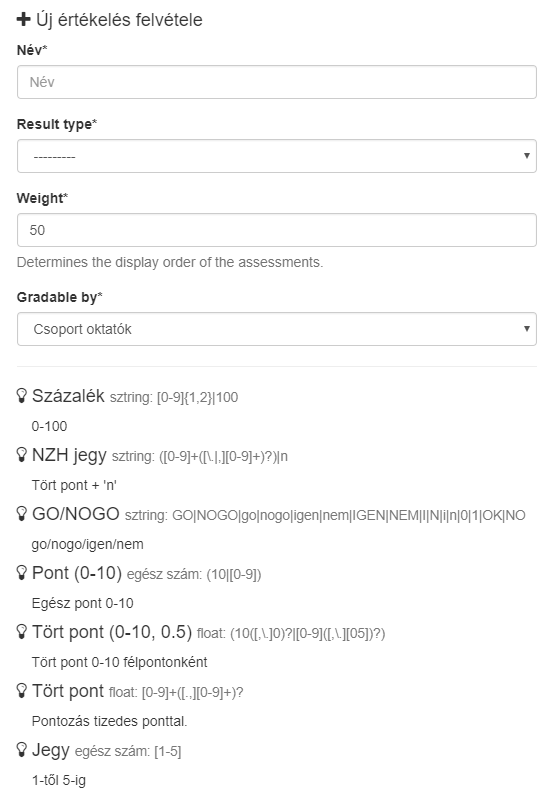
\includegraphics[]{jporta_add_result.png}
    }
    \caption{Értékelés típus hozzáadása}
    \label{fig:jporta_add_result}
\end{figure}

\section{Dinamikus értékelések}\label{section:dynamic-assessments}

Az értékelések létrehozásánál hamar felmerült az igény a dinamikus, azaz automatikusan számolódó mezők használtára. Ezek nagyban megkönnyítik a félév végi összesítést és a végső jegy meghatározását. Viszont ahhoz, hogy ezt széleskörűen lehessen használni egy teljesen általános rendszert kellett fejleszteni, hiszen minden tárgynak eltérő, akár félévről félévre változó követelményei lehetnek, melyekhez más és más számolásokat, súlyozásokat kellhet végezni. 

Ennek megoldására a jelengi implementáció előtt is volt mód, ám az fapadosnak számított. Először az oktatóknak exportálni kellett a meglévő eredményeket egy Excel fájlba, majd ezt a fájlt külső programmal szerkesztve kellett létrehozniuk a dinamikus mezők értékeit. Csak ezután tölthették fel a portálra a bővített fájlt, melynek feldolgozása során a JPorta az ebben található értékeket frissítette. Ezt a módszert Kálmán Viktor cserélte le a jelenlegi alternatívára \cite{KalmanMsc}.

\section{Dinamikus értékelések jelenlegi implementációja}
Az aktuális megvalósításnak két fő követelményt támasztottak: webes felületen beállíthatónak és az oktatók számára könnyen testreszabhatónak kellett lennie.

Ezek teljesítése érdekében a dinamikus mezők kiszámolására Python nyelven írt kódokat használ a portál. Minden dinamikus mezőhöz webes felületen módosítható kód tartozik, amely megkapja a hallgatókhoz tartozó adatokat, majd ez alapján kiszámolja a mező értékét. A megadott Python kódnak tartalmaznia kell egy \textit{calculate\_result} függvényt, mely három szótár (dictionary) típusú paraméterrel rendelkezik:

\begin{enumerate}
    \item paraméter a jelenléteket tartalmazza külön előadás, laboratóriumi és gyakorlati órákra bontva. Minden típushoz megtalálható, hogy hány alkalommal volt jelen a hallgató (attended), hány alkalommal lett megtagadva a jelenléte (denied), hány alkalommal nem jelent meg (no), illetve hogy összesen hány foglalkozás volt tartva abból a típusból (all).
    \item paraméter a (nem dinamikus) értékeléseket taralmazza, \textit{None} értéket ott, ahol nincs megadva eredmény. A kulcs mindig az adott értékelés azonosítója.
    \item paraméterben pedig az automatikusan kiértékelődő feladatok eredményei találhatóak. A kulcs itt is mindig az adott feladat azonosítója, értékei pedig az alábbiak: 
    \begin{itemize}
        \item \textit{None}, ha az adott feladatra nem adott be megoldást a hallgató.
        \item \textit{0}, ha az adott feladat kiértékelés alatt van.
        \item \textit{1}, ha az adott feladat oktatói jóváhagyásra vár.
        \item \textit{2}, ha az adott feladat sikertelen.
        \item \textit{3}, ha az adott feladat sikeresen lefutott.
    \end{itemize}
\end{enumerate}

Ez a függvény minden hallgatóra egyesével fog meghívódni, visszatérési értéke pedig megadja a mező értékét az adott hallgatónál.

Az alábbi példa kód a Programozás alapjai 3. tárgynál használt egyik dinamikus mezőhöz tartozik, feladata a félév végi átlag kiszámítása. Itt a félév során megírt 6 db zárthelyi dolgozatból a legjobb 4 átlagát kell venni, majd kerekíteni 2 tizedesjegyre. A további kerekítést a laborvezető oktatók végzik.

\begin{lstlisting}
def calculate_result(atds, asms, asgs):
    results = [asms[374], asms[375], asms[376], asms[377], asms[378], asms[379]]
    results = [x for x in results if x is not None]
    results.sort(reverse=True)
    return round(sum(results[:4])/4, 2)
\end{lstlisting}

Természetesen a kötelező \textit{calculate\_result} függvény mellett tetszőleges számban használhatunk segédfüggvényeket is a számolás átláthatósága és egyszerűsítése érdekében.

\section{Dinamikus értékelések tesztelése}
Az így elkészített dinamikus mezőben könnyen előfordulhatnak programozói hibák, emiatt a kód felhasználása előtt elengedhetetlen annak átfogó tesztelése. Szerencsére a korábban elkészült rendszer ezt is támogatja. \Aref{fig:jporta_dynamic_test}. ábrán látható módon meg tuduk adni teszt bemeneti paramétereket, majd a rendszer (az eredeti kiértékeléssel megegyező módon) kiszámolja a dinamikus mezőhöz tartozó értéket, így meggyőződhetünk a helyes működéséről.

\begin{figure}[h]
    \centering
    \resizebox{\textwidth}{!}{
        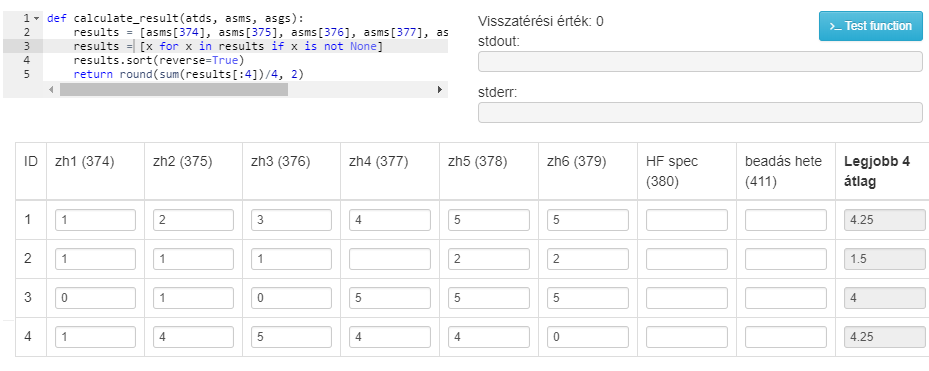
\includegraphics[]{jporta_dynamic_test.png}
    }
    \caption{Dinamikus mező tesztelése}
    \label{fig:jporta_dynamic_test}
\end{figure}

Az értékek mellett láthatjuk a programunk kimeneteit és visszatérési értékét is. Ezeket akár a teszteléshez is felhasználhatjuk, azonban élesítés előtt célszerű ezeket törölni, mivel a portál minden éles futásról tárolja az ilyen jellegű adatokat az ellenőrizhetőség miatt.

Ugyan a példában nem volt szükség sem a jelenlétekre, se az automatikusan kiértékelődő feladatok eredményére, ezeket a számonkérésekhez hasonlóan fel tudjuk használni, illetve a tesztelés is az előzőekkel megegyezően működik.

\section{Dinamikus mezők dinamikus függőségei}